\documentclass{beamer}
\usetheme[pageofpages=de,% String used between the current page and the
                         % total page count.
          bullet=circle,% Use circles instead of squares for bullets.
          titleline=true,% Show a line below the frame title.
          alternativetitlepage=true,% Use the fancy title page.
          titlepagelogo=../img/fse_ministerio_ancho_texto.png%,% Logo for the first page.
	  %watermark=junta_girado,
          %watermarkheight=75px,% Height of the watermark.
          %watermarkheightmult=4,% The watermark image is 4 times bigger
                                % than watermarkheight.
          ]{Torino}

\usepackage[spanish]{babel} % Para separar correctamente las palabras
\usepackage[utf8]{inputenc} % Este paquete permite poner acentos y eñes usando codificación utf-8

\usepackage{color}
\usepackage{listings}


\author{IES Gonzalo Nazareno\\
IES Los Albares\\
IES La Campiña\\
IES Ingeniero de la Cierva\\
\vspace{.5cm}

\includegraphics[width=0.2\textwidth]{cc_by_sa.png}}
\title{OpenStack nova client}
\institute{Proyecto de Innovación\\ {\color{white} .\\} \emph{Implantación y
    puesta a punto de la infraestructura de un cloud computing privado para el
    despliegue de servicios en la nube}}

\definecolor{gray97}{gray}{.97}
\definecolor{gray95}{gray}{.95}
\definecolor{gray90}{gray}{.90}

\lstset{basicstyle=\small,
aboveskip=5pt,
belowskip=5pt
}
%backgroundcolor=\color{fondo}}

\lstdefinestyle{consola}
   {basicstyle=\tiny\bf\ttfamily,
    backgroundcolor=\color{gray90},
   }

\lstdefinestyle{salida}
   {basicstyle=\tiny\ttfamily,
    backgroundcolor=\color{gray95},
   }

\lstdefinestyle{fichero}
   {basicstyle=\tiny\ttfamily,
    xleftmargin=17pt,
    xrightmargin=3pt,
    numbers=left, numberstyle=\tiny, frame=trBL,
    backgroundcolor=\color{gray97},
   }

\begin{document}
\begin{frame}[t,plain]
\titlepage
\end{frame}

\begin{frame}
  \frametitle{Utilización del cliente nova}
  \begin{itemize}
  \item OpenStack Nova, también conocido como OpenStack Compute, es el
    componente principal del Cloud, encargado del manejo de las instancias,
    redes, etc.
  \item De forma análoga a lo presentado en \textit{Introducción a OpenStack
      Horizon}, vamos a realizar las acciones básicas de manejo de instancias,
    pero utilizando en este caso la aplicación \textit{nova} desde línea de
    comandos.
  \item Las acciones que se presentan se realizan con un usuario no privilegiado
    con el rol \textit{member}
  \item Es necesario instalar en el equipo que actúe como cliente el paquete
    \textit{python-novaclient} y obviamente este equipo no tiene que ser un nodo
    del cloud, sólo debe estar conectado a la ``red pública'' del cloud.
  \end{itemize}
\end{frame}

\begin{frame}[fragile]
  \frametitle{Autenticación}
  Es necesario definir varias variables de entorno para poder utilizar
  \textit{nova}, la forma más sencilla es obtener el fichero openrc.sh de
  Horizon:
  \begin{itemize}
  \item \textit{Settings $>$ OpenStack Credentials $>$ Download RC file}
  \end{itemize}
  \begin{lstlisting}[style=consola]
usuario@jupiter:~$ source openrc.sh 
Please enter your OpenStack Password:
  \end{lstlisting}
  \begin{columns}
    \column{.5\textwidth}
    \begin{itemize}
    \item Con lo que se definen en la sesión las variables de entorno:
\begin{lstlisting}[style=salida]
OS_AUTH_URL
OS_TENANT_ID
OS_TENANT_NAME
OS_USERNAME
OS_PASSWORD
\end{lstlisting}
    \end{itemize}
    \column{.5\textwidth}
    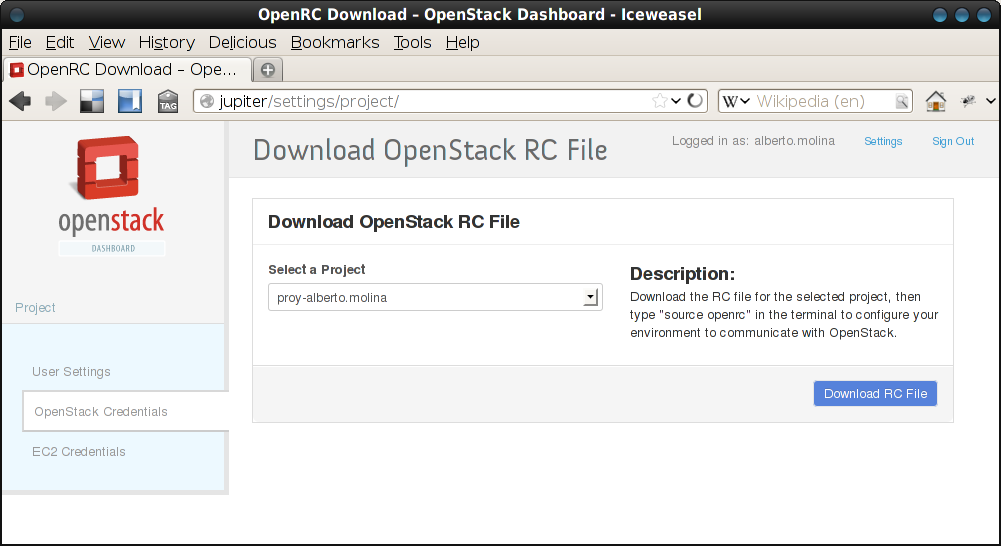
\includegraphics[width=\columnwidth]{../img/nova1.png}
  \end{columns}
\end{frame}

\begin{frame}[fragile]
  \frametitle{Grupos de seguridad}
  Vemos los grupos de seguridad disponibles:
  \begin{lstlisting}[style=consola]
$ nova secgroup-list
+---------+-------------+
|   Name  | Description |
+---------+-------------+
| default | default     |
+---------+-------------+
  \end{lstlisting}
Permitimos todo el protocolo ICMP y ssh (22/tcp) desde la red externa del Cloud
(en este ejemplo la 172.22.0.0/16):
\begin{lstlisting}[style=consola]
$ nova secgroup-add-rule default tcp 22 22 172.22.0.0/16
+-------------+-----------+---------+---------------+--------------+
| IP Protocol | From Port | To Port |    IP Range   | Source Group |
+-------------+-----------+---------+---------------+--------------+
| tcp         | 22        | 22      | 172.22.0.0/16 |              |
+-------------+-----------+---------+---------------+--------------+
\end{lstlisting}
\begin{lstlisting}[style=consola]
$ nova secgroup-add-rule default icmp -1 255 172.22.0.0/16
+-------------+-----------+---------+---------------+--------------+
| IP Protocol | From Port | To Port |    IP Range   | Source Group |
+-------------+-----------+---------+---------------+--------------+
| icmp        | -1        | 255     | 172.22.0.0/16 |              |
+-------------+-----------+---------+---------------+--------------+
\end{lstlisting}
\end{frame}

\begin{frame}[fragile]
  \frametitle{Pares de clave ssh}
  Creamos un par de claves RSA pública/privada en nuestro equipo:
  \begin{lstlisting}[style=consola]
$ cd ~/.ssh
$ ssh-keygen
  \end{lstlisting}
  Añadimos la clave pública al cloud:
  \begin{lstlisting}[style=consola]
$ nova keypair-add --pub_key id_rsa.pub clave-prueba
  \end{lstlisting}
  Listamos las claves públicas disponibles:
    \begin{lstlisting}[style=consola]
$ nova keypair-list
+--------------+-------------------------------------------------+
|     Name     |                   Fingerprint                   |
+--------------+-------------------------------------------------+
| clave-prueba | 11:49:62:78:e3:75:41:29:d9:bd:e1:e9:a7:a7:5d:ed |
| prueba-clase | de:64:6e:2b:0c:85:42:96:46:7d:30:3b:17:e6:66:e0 |
+--------------+-------------------------------------------------+
    \end{lstlisting}
    Y si quisiéramos borrar alguna:
    \begin{lstlisting}[style=consola]
$ nova keypair-delete prueba-clase
    \end{lstlisting}
\end{frame}

\begin{frame}[fragile]
  \frametitle{Listar imágenes y sabores}
  Para ver las imágenes disponibles:
\begin{lstlisting}[style=consola]
$ nova image-list
+--------------------------------------+--------------------------------+--------+-
|                  ID                  |             Name               | Status | 
+--------------------------------------+--------------------------------+--------+-
| 040ec625-baff-4c27-8555-2d4364cab6ce | Debian GNU/Linux wheezy x86_64 | ACTIVE | 
| 1fda706f-61ff-42af-ae4f-f16b459de0e9 | Ubuntu Desktop 12.04 x86_64    | ACTIVE | 
| 5a9977bd-8cff-498b-983d-908702521a37 | Windows 7 Profesional 64bits   | ACTIVE | 
| 69900b94-0bff-4fb1-a7c7-107334100c3a | Ubuntu 12.04 Server x86_64     | ACTIVE | 
| ca0b6cd9-c7ff-4bce-8b08-d118a77f254b | Windows XP                     | ACTIVE | 
| d686f79b-fdff-4ed7-9374-7ca7c955f118 | Debian-KFreeBSD wheezy x86_64  | ACTIVE | 
| fbc88e4c-d1ff-4e6e-b156-6f0554b31236 | Windows 2008 Server R2         | ACTIVE | 
+--------------------------------------+--------------------------------+--------+-
\end{lstlisting}
Para ver los sabores (\textit{flavors}) disponibles:
\begin{lstlisting}[style=consola]
$ nova flavor-list
+----+-----------+-----------+------+-----------+------+-------+-------------+
| ID |    Name   | Memory_MB | Disk | Ephemeral | Swap | VCPUs | RXTX_Factor |
+----+-----------+-----------+------+-----------+------+-------+-------------+
| 1  | m1.tiny   | 512       | 0    | 0         |      | 1     | 1.0         |
| 2  | m1.small  | 2048      | 10   | 20        |      | 1     | 1.0         |
| 3  | m1.medium | 4096      | 10   | 40        |      | 2     | 1.0         |
| 6  | basico    | 512       | 10   | 0         |      | 1     | 1.0         |
+----+-----------+-----------+------+-----------+------+-------+-------------+
\end{lstlisting}
\end{frame}

\begin{frame}[fragile]
  \frametitle{Lanzar instancias (I)}
  Lanzamos una instancia:
\begin{lstlisting}[style=consola]
$ nova boot instancia-1 --image 040ec625-ba8e-4c27-8555-2d4364cab6ce --flavor 6\
 --security_groups default --key_name clave-prueba
+------------------------+--------------------------------------+
| OS-DCF:diskConfig      | MANUAL                               |
| OS-EXT-STS:power_state | 0                                    |
| OS-EXT-STS:task_state  | scheduling                           |
| OS-EXT-STS:vm_state    | building                             |
| accessIPv4             |                                      |
| accessIPv6             |                                      |
| adminPass              | 2P5CK26agTDb                         |
| config_drive           |                                      |
| created                | 2012-10-12T15:50:37Z                 |
| flavor                 | basico                               |
| hostId                 |                                      |
| id                     | 9ff5faaf-a7c3-4374-9ad8-1f47f97dd786 |
| image                  | Debian GNU/Linux wheezy x86_64       |
| key_name               | clave-prueba                         |
| metadata               | {}                                   |
| name                   | instancia-1                          |
| progress               | 0                                    |
| status                 | BUILD                                |
| tenant_id              | ffffffff5894473c8a98f89a895c6b2c     |
| updated                | 2012-10-12T15:50:38Z                 |
| user_id                | aaaaaaaaeecf40f7ac87ec0f93601793     |
+------------------------+--------------------------------------+
\end{lstlisting}
\end{frame}
\begin{frame}[fragile]
  \frametitle{Lanzar instancias (II)}
  Pasados unos instantes comprobamos el estado de la instancia:
\begin{lstlisting}[style=consola]
$ nova show instancia-1
+------------------------+------------------------------------------------------+
| OS-DCF:diskConfig      | MANUAL                                               |
| OS-EXT-STS:power_state | 1                                                    |
| OS-EXT-STS:task_state  | None                                                 |
| OS-EXT-STS:vm_state    | active                                               |
| accessIPv4             |                                                      |
| accessIPv6             |                                                      |
| config_drive           |                                                      |
| created                | 2012-10-12T15:52:57Z                                 |
| flavor                 | basico                                               |
| hostId                 | ffffffffffffff1e734fcf5b555adc7c916c8d67dd435ae55e19 |
| id                     | a11768e4-817b-4103-a5e6-beb0ee615457                 |
| image                  | Debian GNU/Linux wheezy x86_64                       |
| key_name               | clave-prueba                                         |
| metadata               | {}                                                   |
| name                   | instancia-1                                          |
| progress               | 0                                                    |
| status                 | ACTIVE                                               |
| tenant_id              | fffffffff894473c8a98f89a895c6b2c                     |
| updated                | 2012-10-12T15:53:13Z                                 |
| user_id                | aaaaaaaaaecf40f7ac87ec0f93601793                     |
| vlan4 network          | 10.0.4.5                                             |
+------------------------+------------------------------------------------------+
\end{lstlisting}
\end{frame}
\begin{frame}[fragile]
  \frametitle{Asociación de IP flotante}
  En primer lugar solicitamos la asignación de una IP flotante al proyecto
  (\textit{tenant}):
\begin{lstlisting}[style=consola]
$ nova floating-ip-create
+---------------+-------------+----------+------+
|       Ip      | Instance Id | Fixed Ip | Pool |
+---------------+-------------+----------+------+
| 172.22.122.24 | None        | None     | nova |
+---------------+-------------+----------+------+
\end{lstlisting}
Y ahora asociamos esa dirección IP flotante a la instancia:
\begin{lstlisting}[style=consola]
$ nova add-floating-ip instancia-1 172.22.122.24
\end{lstlisting}
\end{frame}

\begin{frame}[fragile]
  \frametitle{Acceso a la instancia}
  Comprobamos la conectividad con la instancia:
\begin{lstlisting}[style=consola]
$ ping -c 3 172.22.122.24
PING 172.22.122.24 (172.22.122.24) 56(84) bytes of data.
64 bytes from 172.22.122.24: icmp_req=1 ttl=63 time=0.771 ms
64 bytes from 172.22.122.24: icmp_req=2 ttl=63 time=0.751 ms
64 bytes from 172.22.122.24: icmp_req=3 ttl=63 time=0.661 ms

--- 172.22.122.24 ping statistics ---
3 packets transmitted, 3 received, 0% packet loss, time 2000ms
rtt min/avg/max/mdev = 0.661/0.727/0.771/0.057 ms
\end{lstlisting}
Y accedemos a la instancia por ssh utilizando la clave RSA privada (en este caso
\texttt{\$HOME/.ssh/id\_rsa} es la clave por defecto):
\begin{lstlisting}[style=consola]
$ ssh root@172.22.122.24
Linux wheezy 3.2.0-3-amd64 #1 SMP Mon Jul 23 02:45:17 UTC 2012 x86_64

The programs included with the Debian GNU/Linux system are free software;
the exact distribution terms for each program are described in the
individual files in /usr/share/doc/*/copyright.

Debian GNU/Linux comes with ABSOLUTELY NO WARRANTY, to the extent
permitted by applicable law.
Last login: Fri Oct 12 18:16:21 2012 from 172.22.3.56
root@wheezy:~# 
\end{lstlisting}
\end{frame}

\begin{frame}[fragile]
Todas las acciones se ejecutan como \texttt{nova <accion> <instancia>}
  \frametitle{Acciones sobre instancias}
  \begin{description}
  \item[delete] Para terminar una instancia
  \item[pause] Para pausar una instancia
  \item[unpause] Para ``des-pausar'' una instancia pausada
  \item[suspend] Para suspender una instancia, almacenar su estado en disco y
    liberar RAM
  \item[resume] Para reanudar una instancia suspendida
  \item[reboot] Para reiniciar una instancia activa
  \item[image-create] Para crear una nueva imagen tomando una instantánea
    (\textit{snapshot}) de una instancia activa
  \item[rename] Para renombrar una instancia
  \end{description}
\end{frame}

\begin{frame}
  \frametitle{Más acciones sobre instancias}
  Las acciones mostradas anteriormente son las mismas que se pueden realizar
  desde el panel de control web Horizon, pero hay más:
  \begin{description}
  \item[resize] Para modificar en ``vivo'' el sabor de una instancia. Permite
    por ejemplo aumentar la RAM de una instancia mientras está activa.
  \item[live-migration] Requiere una configuración particular en la que haya un
    sistema de almacenamiento centralizado de las imágenes de las instancias
    (del directorio \texttt{/var/lib/nova/instances})
  \item[get-vnc-console] Para obtener una URL para conectarse a una consola
    virtual por VNC
  \item[lock] Para bloquear una instancia
  \item[root-password] Para modificar la contraseña de root de la instancia
  \item[unlock] Para desbloquear una instancia
  \end{description}
\end{frame}
\end{document}

